\section{Analiza i specyfikacja wymagań (Bogna Lew)}
W niniejszej sekcji przedstawiono specyfikę wymagań funkcjonalnych, pozafunkcjonalnych oraz tych, wynikających z
głównych założeń projektu. Dodatkowo zawiera ona diagramy przypadków użycia, maszyny stanów oraz klas prototypowej gry.

\subsection{Specyfika wymagań wynikających z założeń projektu}
Z punktu widzenia projektu kluczowe jest jak najdokładniejsze oddanie realiów historycznych przy jednoczesnym
uwzględnieniu jakości rozgrywki gracza oraz cech charakterystycznych dla gier typu RTS. Z założeń wynika, że fabuła
gry powinna zostać osadzona w czasach sprzed wielkich odkryć geograficznych. Na tej podstawie zostały zdefniowane
dodatkowe wymagania, które powinien spełniać prototyp:
\begin{itemize}
  \item Sposób nawigacji powinien jak najdokładniej odpowiadać temu stosowanemu w wybranej epoce
  \item Postacie w grze powinny stylistycznie pasować do realiów historycznych
  \item Postacie powinny posługiwać się słownictwem adekwatnym do czasów, w których osadzona jest gra
  \item Postacie powinny jak najlepiej oddawać światopogląd w danych czasach
  \item Oręż stosowany w grze powinien odpowiadać realiom historycznym
  \item Budowle w grze powinny stylistycznie odpowiadać wybranej epoce
  \item Sposób komunikacji z postaciami powinien imitować ten stosowany w danych czasach
\end{itemize}

\subsection{Wymagania funkcjonalne}\label{ss:fun}
W przedstawionej liście zostały wymienione wymagania funkcjonalne, które powinien spełniać prototyp gry.

\begin{itemize}\label{list:fun}
  \item Zapis oraz odczyt wybranego stanu gry lokalnie na komputerze użytkownika
  \item Uruchomienie nowej gry
  \item Możliwość sterowania postacią gracza
  \item Możliwość nawigacji w świecie gry
  \item Możliwość wchodzenia w interakcję z postaciami niezależnymi
  \item Możliwość przyjmowania zleceń od postaci niezależnych
  \item Możliwość najmowania postaci wojowników
  \item Możliwość wydawania komend wynajętym postaciom
  \item Możliwość zlecania budowy
  \item Możliwość zdobywania zasobów
\end{itemize}

\subsection{Wymagania niefunkcjonalne}\label{ss:nonfun}
Poniższa lista przedstawia wymagania niefunkcjonalne projektu.

\begin{itemize}\label{list:nonfun}
  \item Rozgrywka w trybie offline
  \item Działanie na urządzeniach z systemem Windows lub Linux
  \item Dostosowywanie rozmiaru do wielkości ekranu komputera użytkownika
  \item Obsługa klawiatury oraz myszy
  \item Działanie w czasie rzeczywistym
\end{itemize}

\subsection{Diagram przypadków użycia}\label{ss:usecase}
Niniejsza sekcja przedstawia diagram przypadków użycia dla głównych funkcjonalności, które będzie zawierać prototypowa gra.
Opisuje on przewidywane usługi oferowane przez poszczególne mechaniki programu.
\begin{figure}[!htbp]
    \centering
    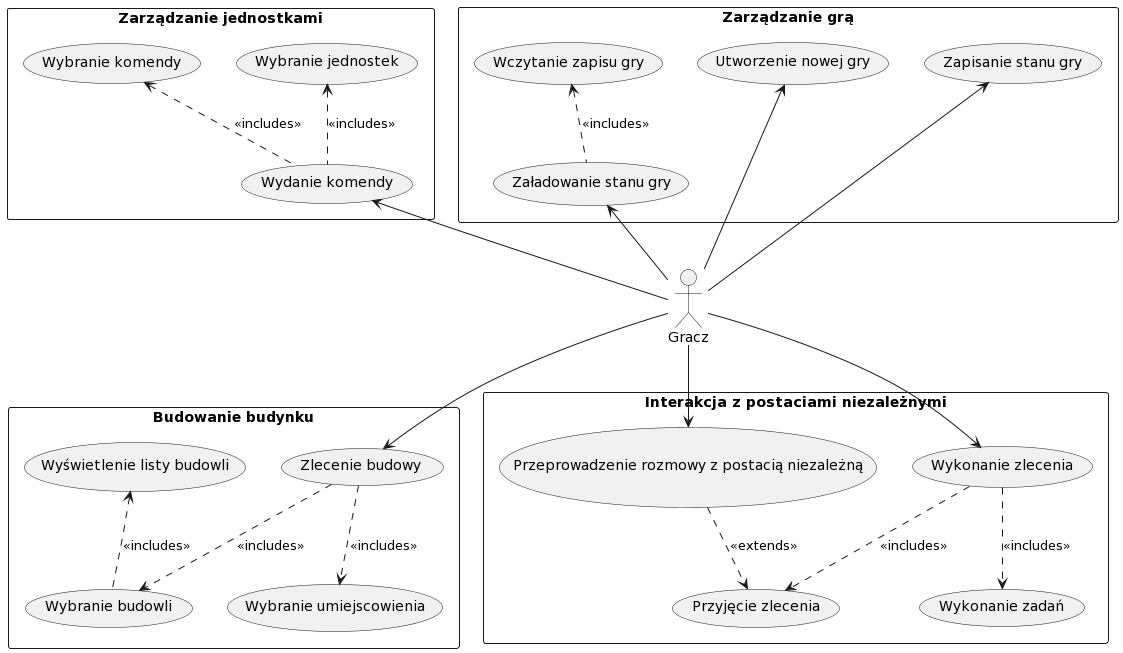
\includegraphics[width=1.0\textwidth]{images/diagrams/usecase.png}
    \caption{Diagram przypadków głównych mechanik gry.}\label{fig:usecases}
\end{figure}
\FloatBarrier

\subsection{Diagram stanów}\label{ss:state}
W tym podpunkcie został przedstawiony diagram stanów prototypowej gry, który ukazuje jej przewidywany sposób działania.
Prezentuje on podstawowe stany, w których może się znaleźć system gry.
\begin{figure}[!htbp]
    \centering
    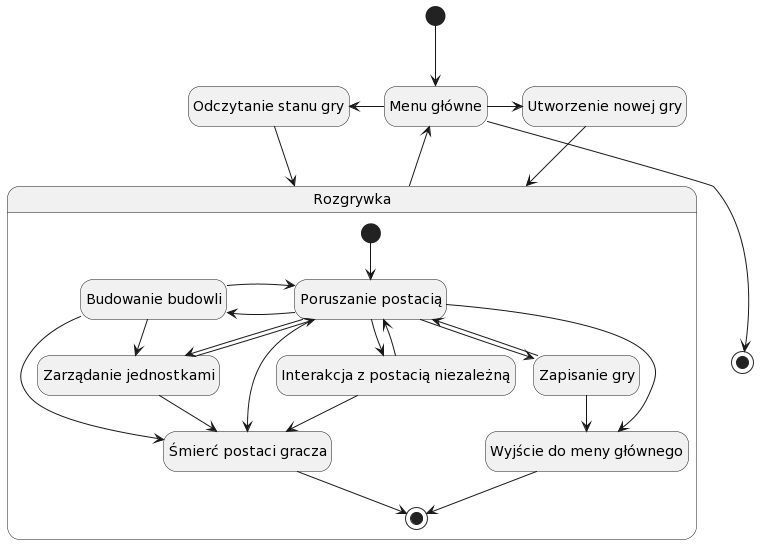
\includegraphics[width=1.0\textwidth]{images/diagrams/state.png}
    \caption{Diagram stanów gry.}\label{fig:states}
\end{figure}
\FloatBarrier

\subsection{Diagram klas}\label{ss:class}
W tej sekcji został pokazany uproszczony diagram klas, przedstawiający główne elementy gry. Obrazuje podstawową
strukturę tworzonego systemu oraz zależności pomiędzy poszczególnymi komponentami.
\begin{figure}[!htbp]
    \centering
    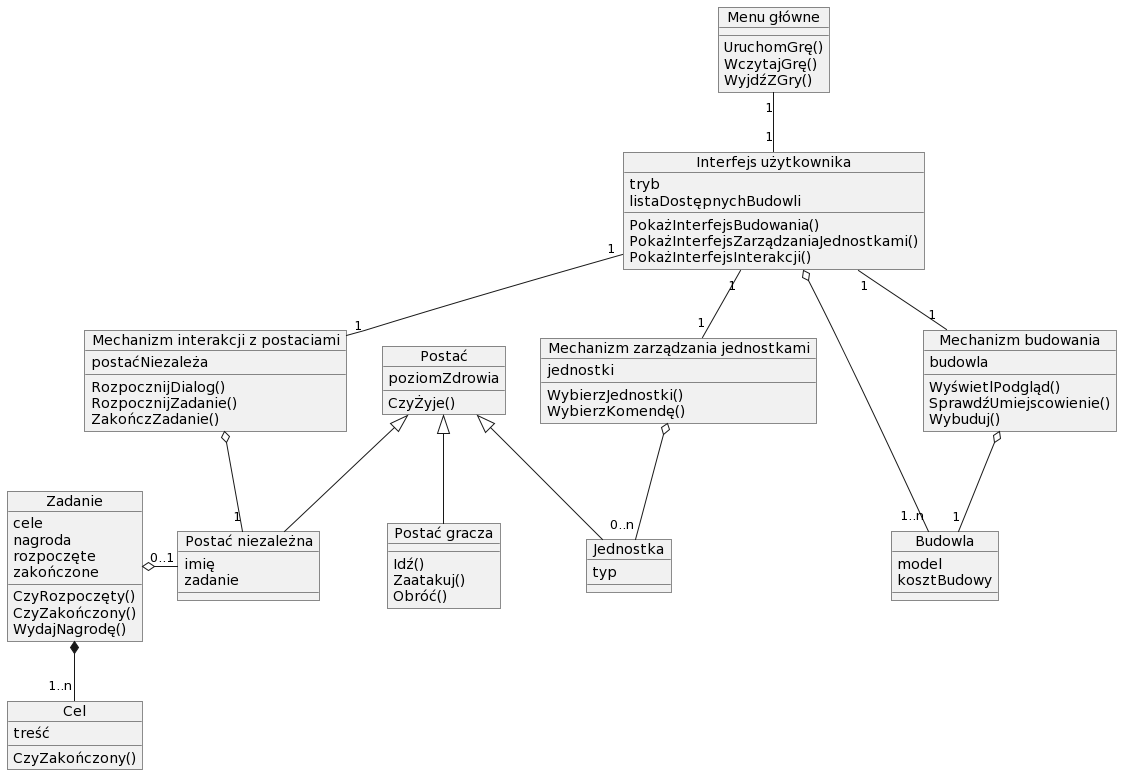
\includegraphics[width=1.0\textwidth]{images/diagrams/class.png}
    \caption{Diagram klas gry.}\label{fig:classes}
\end{figure}